 \newpage

\subsection{Thalliumprobe}
In Tab. \ref{tab:tl} sind die gemessenen Zahlen in Abhängigkeit vom Magnetfeld eingetragen. Daraus wird nun $\eta = a\cdot (U_B - \overline{\delta U})$ und $N' = \frac{N - N_U}{U_B - \overline{\delta U}} \sim \dot{N}$ berechnet (Werte kleiner als 0 wurden auf 0 gesetzt.). Bei letzterem wurde noch durch $U_B - \overline{\delta U}$ geteilt, da aufgrund der Dispersion des Spektrometers der Messwert proportional zum Impuls  der Teilchen ist: $p \sim \eta \sim U_B - \overline{\delta U}$. Aus diesen Werten kann man dann $\varepsilon = \sqrt{1 + \eta^2}$ und $\beta = \frac{\eta}{\varepsilon}$ berechnen. Nun ist nach Gl. \ref{equ:kurie}:
\begin{align*}
Y = \sqrt{\frac{N'}{\eta\varepsilon F_{-}(\eta,82)}}
\end{align*}
Für die Fermifunktion wird $F_{-}(\eta,82)$ eingesetzt, da es sich um einen $\beta^-$-Zerfall handelt und der Restkern (Blei) die Ladungszahl 82 besitzt. Die Fehler werden über Gaußsche Fehlerfortpflanzung berechnet.\\

In Abb. \ref{fig:tl} ist der Kurieplot abgebildet. Es wurde ein linearer Fit $Y = m \epsilon + n$ in dem linearem Bereich $1,35 < \varepsilon < 2,3$ durchgeführt. Dieser ergab:
\begin{align*}
m &= -\si{(0,6\pm 0,02)}\\
n &= \si{(1,38 \pm 0,04)}
\end{align*}
Damit ergibt sich $\varepsilon_0 = -\frac{n}{m} = 2,3 \pm 0,1$. Das entspricht einer kinetischen Energie von:
\begin{align*}
E_\mathrm{Tl} = (\varepsilon_0 - 1)\cdot m_ec^2 = \si{(0,67 \pm 0,05)\mega\eV}
\end{align*}

Der Literaturwert \cite{tlenergy} liegt bei $\SI{0,76}{\mega\eV}$. Dieser Wert liegt nah an dem Ergebnis unserer Messung, aber außerhalb des Fehlerintervalls. Da auch der Wert für Natrium kleiner als der Literaturwert ist, vermuten wir, dass es sich um einen systematischen Fehler handelt, z.B., dass der nur einmal gemessene Untergrund $N_2$ zu hoch war. Dadurch werden die Y-Werte kleiner, was die Kurve nach unten verschiebt und somit eine kleinere Maximalenergie gemessen wird.  

\begin{figure}[h]
\centering
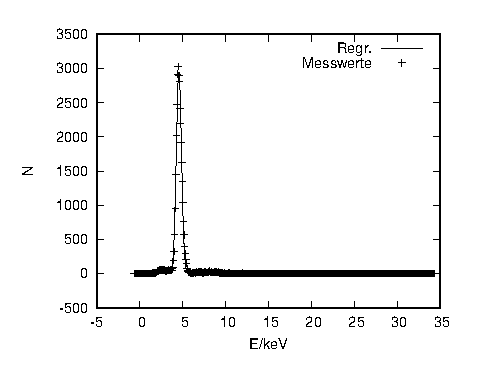
\includegraphics[width=0.75\linewidth]{data/ti.eps}
\caption{Kurieplot für Thallium}
\label{fig:tl}
\end{figure}

\newpage

\subsection{Natriumprobe}
Es wird nun $Y$ analog wie bei der Thalliumprobe berechnet. Für die Fermifunktion verwendet man nun $F_+(\eta, 10)$, da der $\beta^+$-Zerfall zu einem Neonkern führt (Kernladungszahl 10).\\

In Abb. \ref{fig:na} ist der Kurieplot abgebildet. Es wurde ein linearer Fit $Y = m \epsilon + n$ in dem linearem Bereich $1,2 < \varepsilon < 2$ durchgeführt. Dieser ergab:
\begin{align*}
m &= -\si{(2,7\pm 0,2)}\\
n &= \si{(5,3 \pm 0,2)}
\end{align*}

Damit ergibt sich $\varepsilon_0 = -\frac{n}{m} = 2 \pm 0,1$. Das entspricht einer kinetischen Energie von:
\begin{align*}
E_\mathrm{Na} = (\varepsilon_0 - 1)\cdot m_ec^2 = \si{(0,51 \pm 0,05)\mega\eV}
\end{align*}

Dieser Wert stimmt im Rahmen des Fehlers mit dem Literaturwert\cite{naenergy} von $\SI{0,545}{\mega\eV}$ überein.

\begin{figure}[h]
\centering
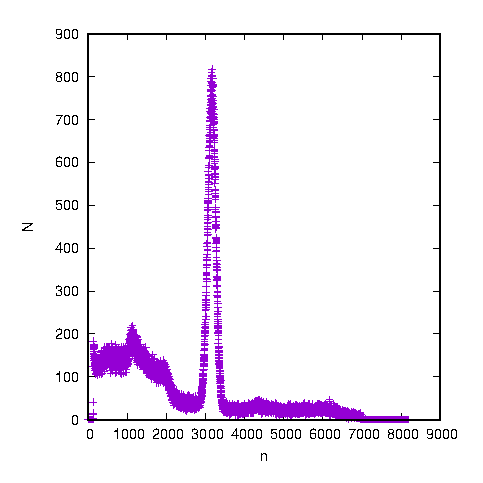
\includegraphics[width=0.75\linewidth]{data/na.eps}
\caption{Kurieplot für Natrium}
\label{fig:na}
\end{figure}
